\documentclass[10.5pt,a4paper]{article}
\usepackage[margin=19mm,top=20mm,bottom=20mm]{geometry}
\usepackage{graphicx}
\usepackage{booktabs}
\usepackage{tabularx}
\usepackage{xcolor}
\usepackage{fancyhdr}
\usepackage{caption}
\usepackage{enumitem}
\usepackage{hyperref}

\definecolor{SnapPurple}{HTML}{6E56CF}
\definecolor{SnapDark}{HTML}{1B2030}
\definecolor{SnapMuted}{HTML}{596579}
\definecolor{SnapLight}{HTML}{F3F1FA}

\hypersetup{
  colorlinks=true,
  linkcolor=SnapPurple,
  urlcolor=SnapPurple,
  citecolor=SnapPurple,
  pdftitle={SnapFix: AI-assisted Home Repair with Manual Evidence},
  pdfauthor={COMP7506 SnapFix Team}
}

\pagestyle{fancy}
\fancyhf{}
\fancyhead[L]{\small\color{SnapMuted}COMP7506 Group Project}
\fancyhead[R]{\small\color{SnapMuted}SnapFix}
\fancyfoot[C]{\small\thepage}
\setlength{\parindent}{0pt}
\setlength{\parskip}{5pt}
\setlist{noitemsep,topsep=3pt}
\sloppy

\title{
  \vspace{-12mm}
  {\color{SnapPurple}\Huge\bfseries SnapFix}\\[4mm]
  {\Large\bfseries AI-assisted Home Repair with Manual Evidence}\\[3mm]
  {\large\color{SnapMuted}Photo diagnosis, safety decisions, repair tracking and bilingual reporting}
}
\author{COMP7506 Group Project}
\date{Initial report draft · November 2026}

\begin{document}
\maketitle
\thispagestyle{empty}

\begin{center}
\begin{tabular}{ll}
\toprule
\textbf{Member} & \textbf{Student ID} \\
\midrule
Cao Junjia & \\
Shi Junying & \\
Zhu Yutaimin & \\
Yang Ruijia & \\
Zhang Fan & \\
\bottomrule
\end{tabular}
\end{center}

\vspace{3mm}
\begin{abstract}
SnapFix is a smart-home maintenance application for tenants and household users who can observe a problem but may not know the appliance model, relevant instructions, or safest next step. The application combines Qwen3-VL visual extraction, BM25 manual retrieval, deterministic safety rules, chunk-level citation validation, persistent repair progress, and editable Chinese/English repair requests. Rather than treating a model response as authoritative, SnapFix separates visible observations from possible causes and withholds unsupported do-it-yourself instructions. The current implementation includes real accounts, source-linked guidance, safety refusal, and a repair archive. Evaluation covers 46 backend tests, five Flutter tests, 26 controlled image-quality variants, and selected real Qwen workflows. These results demonstrate implementation and workflow reliability; they do not establish universal diagnostic accuracy.
\end{abstract}

\vspace{2mm}
{\small\textbf{Keywords:} smart home, appliance repair, multimodal AI, retrieval-augmented generation, safety, mobile application}

\newpage
\section{Background Research}

\subsection{Market context}

Household repair guidance is distributed across repair communities, visual search tools, and professional consultation services. Each addresses a different part of the user journey, but a tenant still needs to connect device identity, applicable instructions, safety, and communication with a landlord or technician. Our comparison is based on published product documentation, not a controlled hands-on reliability comparison.

\begin{center}
\small
\begin{tabularx}{\textwidth}{p{29mm}X X}
\toprule
\textbf{Application} & \textbf{Documented capabilities} & \textbf{Design question relevant to SnapFix} \\
\midrule
iFixit / FixBot & Step-by-step repair guides, a repair knowledge base, and visual assistance through questions and photos. \cite{ifixit} & Users still need to confirm that guidance applies to their exact device. SnapFix keeps model identity, uncertainty, and evidence visible. \\
\addlinespace[3pt]
Frontdoor & Video consultations with repair experts, saved call notes, and referrals to local professionals. \cite{frontdoor} & Live consultation depends on connectivity, expert availability, and regional coverage. SnapFix prepares a concise bilingual request before contact. \\
\addlinespace[3pt]
Google Lens & Visual search for objects, similar images, related websites, and AI overviews. \cite{lens} & Visual similarity alone does not establish a model-specific fault or validated procedure. SnapFix uses visual extraction as an input to retrieval, not as sufficient repair evidence. \\
\bottomrule
\end{tabularx}
\end{center}

The open-source FixIt Lens project is an additional engineering reference for image input, retrieval, safety checks, and evaluation; it is not counted as one of the three market applications above. \cite{fixitlens}

\subsection{Opportunity}

The opportunity is the integration of a narrow rental workflow rather than a claim that any individual capability is unique. SnapFix collects device information, presents supporting instructions, decides whether professional help is appropriate, and prepares a repair request in Chinese or English. The intended user value is a clear and traceable next step, especially when a tenant cannot safely or confidently perform a repair.

\section{Application Overview}

\subsection{Category and motivation}

SnapFix is an \textbf{information and household maintenance application}. Its target users are students and tenants who encounter unfamiliar appliances, missing manuals, or error codes. Three recurring problems motivate the design:

\begin{enumerate}
  \item A user can see a warning light or error code but cannot reliably identify the applicable instruction.
  \item A user may not know whether a task is non-destructive, model-specific, or dangerous.
  \item After deciding to seek help, the user still needs to describe the device, observed issue, attempted steps, and safety concerns clearly.
\end{enumerate}

The product principle is therefore \textbf{``Snap it. Fix it. Or report it.''} Diagnosis is not treated as complete until the user receives either evidence-linked guidance or a safe route to professional help.

\subsection{Design and features}

The mobile flow supports camera or library input, a manual error-code path, analysis progress, a diagnosis report, step feedback, repair status, an archive, and bilingual repair drafts. The interface supports English and Simplified Chinese, light/dark/system appearance, and reduced motion. Real accounts support email, Sign in with Apple, and Google OAuth, with per-user isolation of sessions and preferences.

\begin{center}
\begin{tabularx}{\textwidth}{l X}
\toprule
\textbf{Feature} & \textbf{Delivered behavior} \\
\midrule
Photo diagnosis & Extracts device category, brand, model, error code, visible symptoms, and confidence without requiring unknown fields. \\
Manual lookup & Accepts brand and error-code input without requiring a camera. \\
Grounded steps & Displays exact manual chunks, original excerpts, PDF pages, and source URLs. \\
Safety guardrails & Applies deterministic rules before generation and again to generated steps. \\
Repair progress & Persists done, skipped, and not-useful feedback; repeated taps undo feedback. \\
Repair status & Supports investigating, awaiting-repair, and resolved states with archive filters. \\
Bilingual reports & Allows editing, saving, resetting, copying, and sharing Chinese or English drafts. \\
Explicit demo mode & Uses labelled deterministic scenarios without model credentials; unknown images are rejected. \\
\bottomrule
\end{tabularx}
\end{center}

\begin{figure}[htbp]
  \centering
  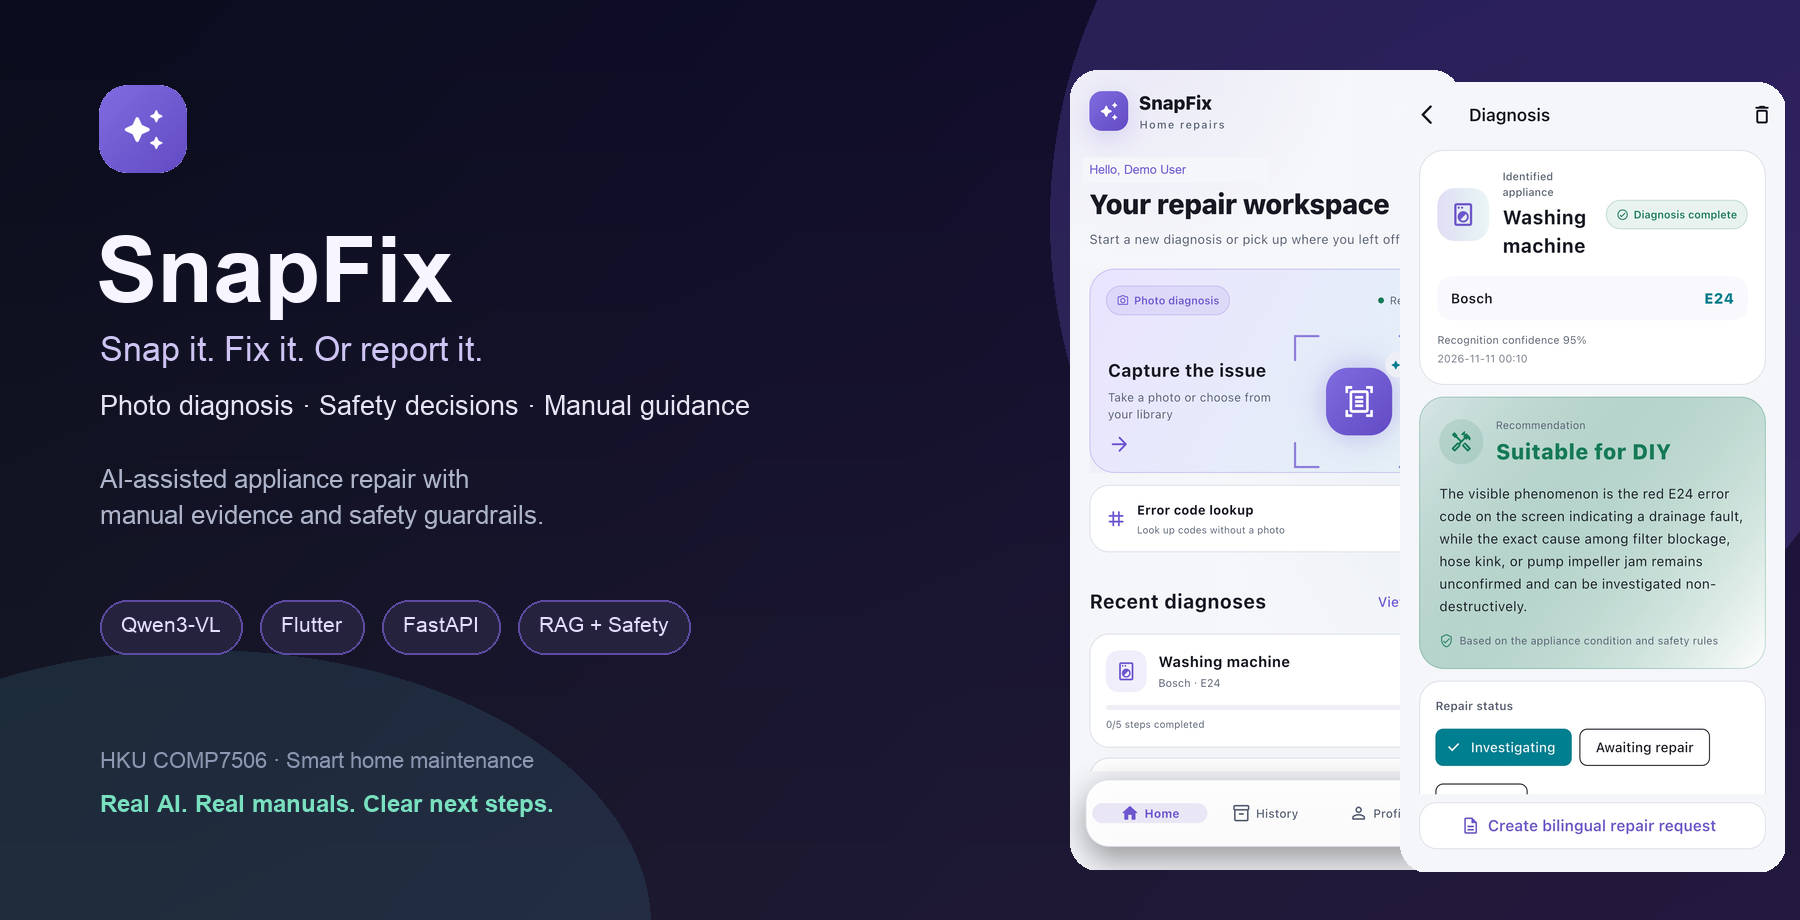
\includegraphics[width=\textwidth]{../assets/snapfix-hero.png}
  \caption{SnapFix product overview with real application screens. Personal information in the home screenshot is replaced by a demo label.}
\end{figure}

\section{System and AI Design}

\subsection{Architecture}

SnapFix uses a Flutter application and an authenticated FastAPI backend. Qwen3-VL is the currently verified live provider through an OpenAI-compatible API; Gemini remains an optional provider. SQLite stores user accounts, token hashes, diagnoses, step feedback, repair status, report drafts, and the imported manual corpus. Original photographs are not written to the database.

\begin{figure}[htbp]
  \centering
  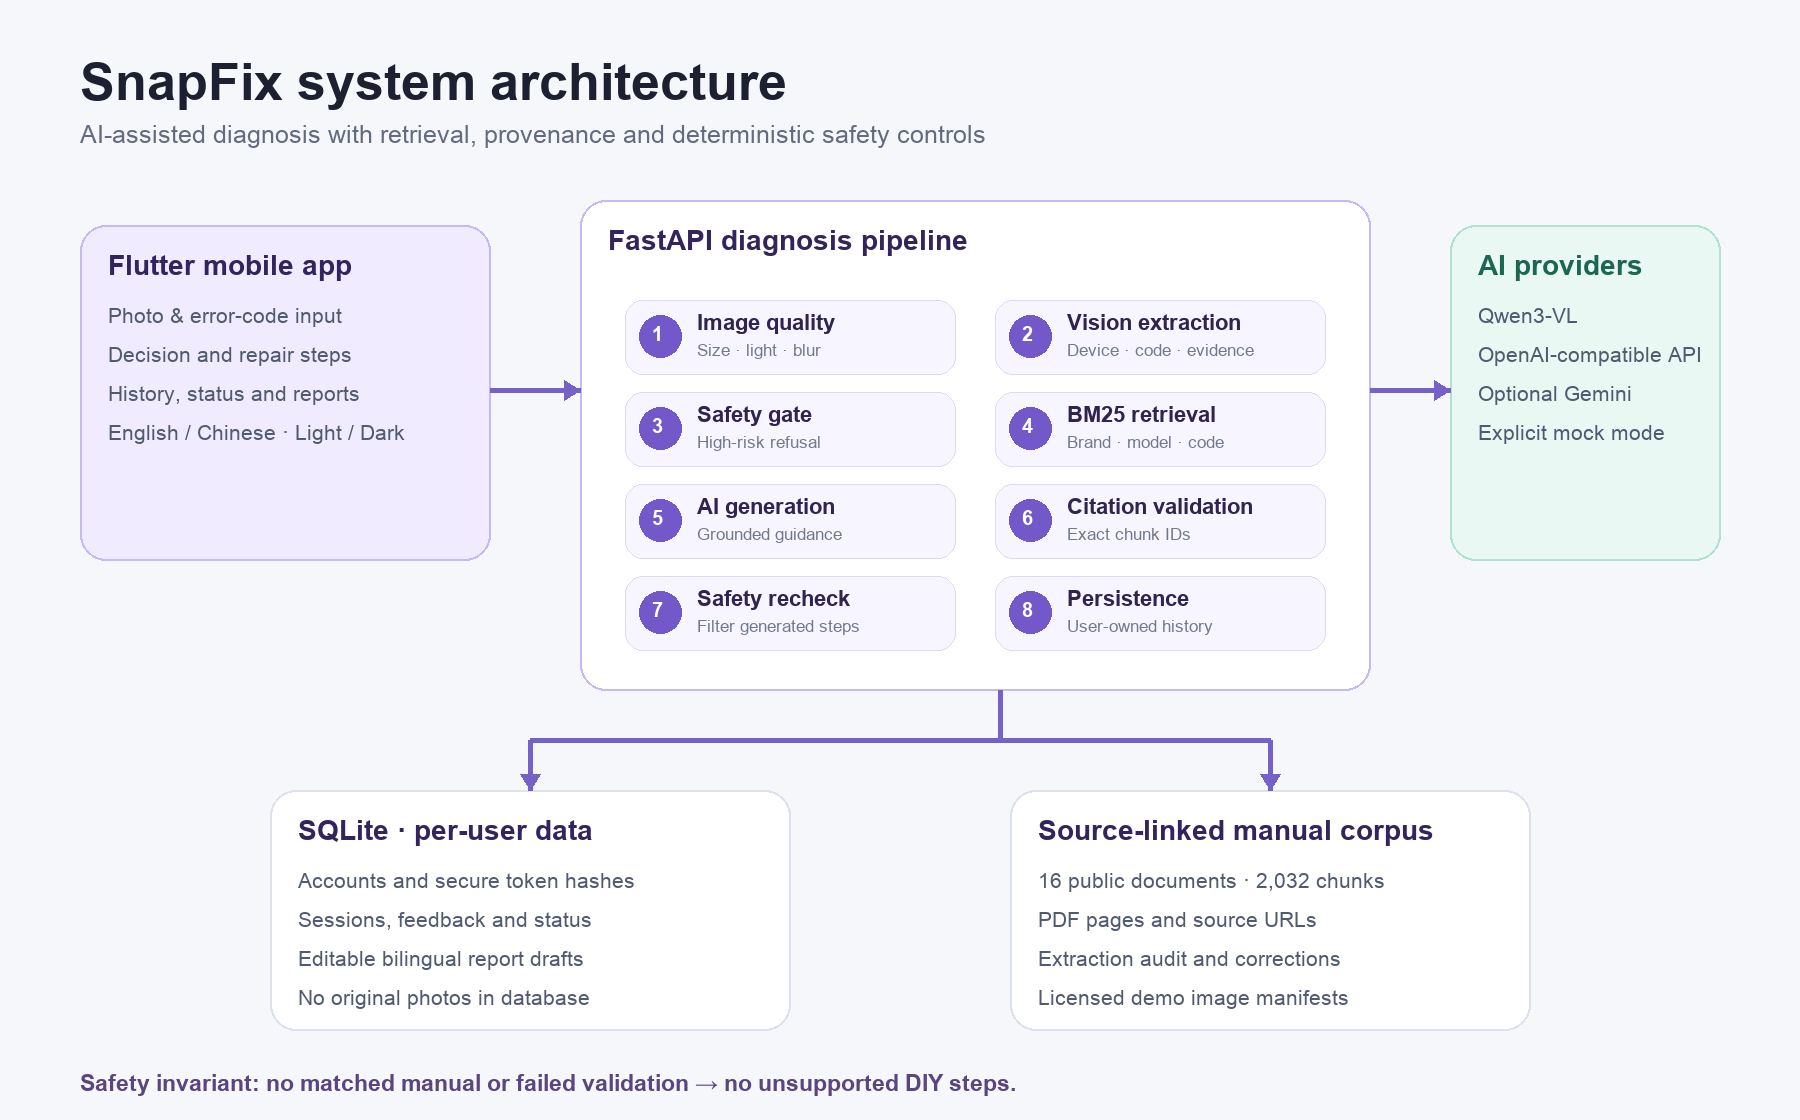
\includegraphics[width=\textwidth]{../assets/architecture.png}
  \caption{System architecture and the separation of AI generation from deterministic safety and evidence validation.}
\end{figure}

\subsection{Diagnosis pipeline}

\begin{enumerate}
  \item \textbf{Image quality.} Validate file size, dimensions, brightness, sharpness, and readability before model invocation.
  \item \textbf{Vision extraction.} Produce structured JSON for device identity and visible observations. The prompt prohibits invented models, error codes, or internal faults.
  \item \textbf{Safety gate.} Refuse high-risk categories before generation, including mains electricity, gas, refrigerant, lithium batteries, pressure equipment, and microwave components.
  \item \textbf{BM25 retrieval.} Rank real manual chunks using category filters, brand aliases, bilingual expansion, and normalized error codes.
  \item \textbf{Grounded generation.} Request a decision and steps constrained to retrieved evidence and the current interface language.
  \item \textbf{Citation validation.} Accept only exact chunk IDs from the retrieval result and preserve original text and PDF pages.
  \item \textbf{Generated-content safety review.} Drop generated steps that introduce dangerous operations even when a citation is present.
  \item \textbf{Persistence.} Save the resulting session and subsequent repair activity under the authenticated user.
\end{enumerate}

This design deliberately separates probabilistic model output from deterministic safety and evidence checks. Low-confidence recognition, missing manual coverage, invalid citations, and unsafe generated content all lead to an explicit non-DIY outcome. A live provider failure returns an error and never substitutes an unrelated mock diagnosis.

\section{Implementation and Evaluation}

\subsection{Corpus and provenance}

The current corpus contains 16 public documents and 2,032 text chunks. Records include source URLs, PDF pages, stable chunk IDs, source hashes, and extraction metadata. The extraction audit records sparse and undecodable pages, while source-bound corrections remain linked to the original file hash. Public demonstration photographs include author, licence, hash, and usage metadata. Appearance images are used for workflow and image-quality testing, not as confirmed fault examples.

\subsection{Current verification}

\begin{center}
\small
\begin{tabularx}{\textwidth}{p{37mm} p{27mm} X}
\toprule
\textbf{Verification} & \textbf{Current result} & \textbf{Scope} \\
\midrule
Backend regression & 46 passed & Corpus, retrieval, safety, image quality, account isolation, status, and report drafts \\
Flutter tests & 5 passed & Model parsing and product interaction logic \\
Flutter analysis & No issues found & Static Dart checks, not device compatibility \\
Image-quality variants & 26 controlled cases & Dark/blur retake behavior, not diagnostic accuracy \\
Real Qwen HTTP flows & Router, microwave, Bosch E24 & Live provider integration and source validation on those scenarios \\
Manual corpus & 16 documents / 2,032 chunks & Available evidence coverage, not universal appliance support \\
\bottomrule
\end{tabularx}
\end{center}

The backend suite uses an isolated temporary database and does not call a live model. Flutter tests cover model parsing, source expansion, feedback and undo, status confirmation, and report editing across language switches. Real HTTP checks confirmed Qwen source labels, microwave safety refusal, an English safety report, and Bosch E24 guidance linked to real manual chunks.

\subsection{Limitations}

The current build is a course project and local development deployment, not a public repair service. The corpus covers a limited set of devices, and the present evaluation does not establish broad fault-recognition accuracy. Camera permissions, notifications, system sharing, and OAuth still require physical-device validation. Future work should expand confirmed-fault photographs, improve manual coverage, evaluate a larger labelled dataset, and add production monitoring and public privacy documentation without weakening citation or safety requirements.

\section{Contributions}

The Solo mainline integrates selected outputs from the original team workstreams. The table records the original team roles and the sources referenced by the integrated repository; it does not imply that every team feature was merged unchanged.

\begin{center}
\small
\begin{tabularx}{\textwidth}{p{25mm} p{34mm} X}
\toprule
\textbf{Member} & \textbf{Original role} & \textbf{Workstream and coordination responsibilities} \\
\midrule
Cao Junjia & Team lead; BE-1 pipeline & Team planning and task coordination; backend architecture, API contracts, providers and safety; integration review, PR coordination, and submission planning \\
Shi Junying & BE-2 retrieval and storage & BM25 retrieval, SQLite persistence, reporting endpoints, and backend documentation \\
Zhu Yutaimin & FE-1 scan and diagnosis & Flutter foundations, shared components, home, camera, preview, and diagnosis flow \\
Yang Ruijia & FE-2 guidance and archive & Step guidance, repair history, report interactions, visual design, and video materials \\
Zhang Fan & Data and content & Corpus ETL, demonstration scenarios, market research, acceptance records, and attributed image assets \\
\bottomrule
\end{tabularx}
\end{center}

Each member should confirm the final description and add work completed outside GitHub before submission. Each member of a multi-person team must also submit the course Peer Review Form separately.

\begin{thebibliography}{9}
\bibitem{ifixit}
iFixit, ``Introducing FixBot,'' 9 December 2025. \url{https://www.ifixit.com/News/114700/introducing-fixbot}. Reviewed 30 October 2026.

\bibitem{frontdoor}
Frontdoor, application support and FAQ. \url{https://www.frontdoor.com/member-support}; Android application listing: \url{https://play.google.com/store/apps/details?id=com.frontdoor.app.prod}. Reviewed 30 October 2026.

\bibitem{lens}
Google Search Help, ``Search with an image on Google.'' \url{https://support.google.com/websearch/answer/1325808?hl=en}. Reviewed 30 October 2026.

\bibitem{fixitlens}
FixIt Lens repository, engineering reference. \url{https://github.com/rakexhs/fixit-lens}. Reviewed 30 October 2026.
\end{thebibliography}

\end{document}
